
%% bare_conf.tex
%% V1.3
%% 2007/01/11
%% by Michael Shell
%% See:
%% http://www.michaelshell.org/
%% for current contact information.
%%
%% This is a skeleton file demonstrating the use of IEEEtran.cls
%% (requires IEEEtran.cls version 1.7 or later) with an IEEE conference paper.
%%
%% Support sites:
%% http://www.michaelshell.org/tex/ieeetran/
%% http://www.ctan.org/tex-archive/macros/latex/contrib/IEEEtran/
%% and
%% http://www.ieee.org/

%%*************************************************************************
%% Legal Notice:
%% This code is offered as-is without any warranty either expressed or
%% implied; without even the implied warranty of MERCHANTABILITY or
%% FITNESS FOR A PARTICULAR PURPOSE! 
%% User assumes all risk.
%% In no event shall IEEE or any contributor to this code be liable for
%% any damages or losses, including, but not limited to, incidental,
%% consequential, or any other damages, resulting from the use or misuse
%% of any information contained here.
%%
%% All comments are the opinions of their respective authors and are not
%% necessarily endorsed by the IEEE.
%%
%% This work is distributed under the LaTeX Project Public License (LPPL)
%% ( http://www.latex-project.org/ ) version 1.3, and may be freely used,
%% distributed and modified. A copy of the LPPL, version 1.3, is included
%% in the base LaTeX documentation of all distributions of LaTeX released
%% 2003/12/01 or later.
%% Retain all contribution notices and credits.
%% ** Modified files should be clearly indicated as such, including  **
%% ** renaming them and changing author support contact information. **
%%
%% File list of work: IEEEtran.cls, IEEEtran_HOWTO.pdf, bare_adv.tex,
%%                    bare_conf.tex, bare_jrnl.tex, bare_jrnl_compsoc.tex
%%*************************************************************************

% *** Authors should verify (and, if needed, correct) their LaTeX system  ***
% *** with the testflow diagnostic prior to trusting their LaTeX platform ***
% *** with production work. IEEE's font choices can trigger bugs that do  ***
% *** not appear when using other class files.                            ***
% The testflow support page is at:
% http://www.michaelshell.org/tex/testflow/



% Note that the a4paper option is mainly intended so that authors in
% countries using A4 can easily print to A4 and see how their papers will
% look in print - the typesetting of the document will not typically be
% affected with changes in paper size (but the bottom and side margins will).
% Use the testflow package mentioned above to verify correct handling of
% both paper sizes by the user's LaTeX system.
%
% Also note that the "draftcls" or "draftclsnofoot", not "draft", option
% should be used if it is desired that the figures are to be displayed in
% draft mode.
%
\documentclass[conference]{IEEEtran}
% Add the compsoc option for Computer Society conferences.
%
% If IEEEtran.cls has not been installed into the LaTeX system files,
% manually specify the path to it like:
% \documentclass[conference]{../sty/IEEEtran}





% Some very useful LaTeX packages include:
% (uncomment the ones you want to load)


% *** MISC UTILITY PACKAGES ***
%
%\usepackage{ifpdf}
% Heiko Oberdiek's ifpdf.sty is very useful if you need conditional
% compilation based on whether the output is pdf or dvi.
% usage:
% \ifpdf
%   % pdf code
% \else
%   % dvi code
% \fi
% The latest version of ifpdf.sty can be obtained from:
% http://www.ctan.org/tex-archive/macros/latex/contrib/oberdiek/
% Also, note that IEEEtran.cls V1.7 and later provides a builtin
% \ifCLASSINFOpdf conditional that works the same way.
% When switching from latex to pdflatex and vice-versa, the compiler may
% have to be run twice to clear warning/error messages.






% *** CITATION PACKAGES ***
%
\usepackage{cite}
% cite.sty was written by Donald Arseneau
% V1.6 and later of IEEEtran pre-defines the format of the cite.sty package
% \cite{} output to follow that of IEEE. Loading the cite package will
% result in citation numbers being automatically sorted and properly
% "compressed/ranged". e.g., [1], [9], [2], [7], [5], [6] without using
% cite.sty will become [1], [2], [5]--[7], [9] using cite.sty. cite.sty's
% \cite will automatically add leading space, if needed. Use cite.sty's
% noadjust option (cite.sty V3.8 and later) if you want to turn this off.
% cite.sty is already installed on most LaTeX systems. Be sure and use
% version 4.0 (2003-05-27) and later if using hyperref.sty. cite.sty does
% not currently provide for hyperlinked citations.
% The latest version can be obtained at:
% http://www.ctan.org/tex-archive/macros/latex/contrib/cite/
% The documentation is contained in the cite.sty file itself.






% *** GRAPHICS RELATED PACKAGES ***
%
\ifCLASSINFOpdf
  \usepackage[pdftex]{graphicx}
  % declare the path(s) where your graphic files are
  % \graphicspath{{../pdf/}{../jpeg/}}
  % and their extensions so you won't have to specify these with
  % every instance of \includegraphics
  % \DeclareGraphicsExtensions{.pdf,.jpeg,.png}
\else
  % or other class option (dvipsone, dvipdf, if not using dvips). graphicx
  % will default to the driver specified in the system graphics.cfg if no
  % driver is specified.
  % \usepackage[dvips]{graphicx}
  % declare the path(s) where your graphic files are
  % \graphicspath{{../eps/}}
  % and their extensions so you won't have to specify these with
  % every instance of \includegraphics
  % \DeclareGraphicsExtensions{.eps}
\fi
% graphicx was written by David Carlisle and Sebastian Rahtz. It is
% required if you want graphics, photos, etc. graphicx.sty is already
% installed on most LaTeX systems. The latest version and documentation can
% be obtained at: 
% http://www.ctan.org/tex-archive/macros/latex/required/graphics/
% Another good source of documentation is "Using Imported Graphics in
% LaTeX2e" by Keith Reckdahl which can be found as epslatex.ps or
% epslatex.pdf at: http://www.ctan.org/tex-archive/info/
%
% latex, and pdflatex in dvi mode, support graphics in encapsulated
% postscript (.eps) format. pdflatex in pdf mode supports graphics
% in .pdf, .jpeg, .png and .mps (metapost) formats. Users should ensure
% that all non-photo figures use a vector format (.eps, .pdf, .mps) and
% not a bitmapped formats (.jpeg, .png). IEEE frowns on bitmapped formats
% which can result in "jaggedy"/blurry rendering of lines and letters as
% well as large increases in file sizes.
%
% You can find documentation about the pdfTeX application at:
% http://www.tug.org/applications/pdftex


\usepackage{color}



% *** MATH PACKAGES ***
%
\usepackage[cmex10]{amsmath}
% A popular package from the American Mathematical Society that provides
% many useful and powerful commands for dealing with mathematics. If using
% it, be sure to load this package with the cmex10 option to ensure that
% only type 1 fonts will utilized at all point sizes. Without this option,
% it is possible that some math symbols, particularly those within
% footnotes, will be rendered in bitmap form which will result in a
% document that can not be IEEE Xplore compliant!
%
% Also, note that the amsmath package sets \interdisplaylinepenalty to 10000
% thus preventing page breaks from occurring within multiline equations. Use:
%\interdisplaylinepenalty=2500
% after loading amsmath to restore such page breaks as IEEEtran.cls normally
% does. amsmath.sty is already installed on most LaTeX systems. The latest
% version and documentation can be obtained at:
% http://www.ctan.org/tex-archive/macros/latex/required/amslatex/math/





% *** SPECIALIZED LIST PACKAGES ***
%
%\usepackage{algorithmic}
% algorithmic.sty was written by Peter Williams and Rogerio Brito.
% This package provides an algorithmic environment fo describing algorithms.
% You can use the algorithmic environment in-text or within a figure
% environment to provide for a floating algorithm. Do NOT use the algorithm
% floating environment provided by algorithm.sty (by the same authors) or
% algorithm2e.sty (by Christophe Fiorio) as IEEE does not use dedicated
% algorithm float types and packages that provide these will not provide
% correct IEEE style captions. The latest version and documentation of
% algorithmic.sty can be obtained at:
% http://www.ctan.org/tex-archive/macros/latex/contrib/algorithms/
% There is also a support site at:
% http://algorithms.berlios.de/index.html
% Also of interest may be the (relatively newer and more customizable)
% algorithmicx.sty package by Szasz Janos:
% http://www.ctan.org/tex-archive/macros/latex/contrib/algorithmicx/




% *** ALIGNMENT PACKAGES ***
%
%\usepackage{array}
% Frank Mittelbach's and David Carlisle's array.sty patches and improves
% the standard LaTeX2e array and tabular environments to provide better
% appearance and additional user controls. As the default LaTeX2e table
% generation code is lacking to the point of almost being broken with
% respect to the quality of the end results, all users are strongly
% advised to use an enhanced (at the very least that provided by array.sty)
% set of table tools. array.sty is already installed on most systems. The
% latest version and documentation can be obtained at:
% http://www.ctan.org/tex-archive/macros/latex/required/tools/


%\usepackage{mdwmath}
%\usepackage{mdwtab}
% Also highly recommended is Mark Wooding's extremely powerful MDW tools,
% especially mdwmath.sty and mdwtab.sty which are used to format equations
% and tables, respectively. The MDWtools set is already installed on most
% LaTeX systems. The lastest version and documentation is available at:
% http://www.ctan.org/tex-archive/macros/latex/contrib/mdwtools/


% IEEEtran contains the IEEEeqnarray family of commands that can be used to
% generate multiline equations as well as matrices, tables, etc., of high
% quality.


%\usepackage{eqparbox}
% Also of notable interest is Scott Pakin's eqparbox package for creating
% (automatically sized) equal width boxes - aka "natural width parboxes".
% Available at:
% http://www.ctan.org/tex-archive/macros/latex/contrib/eqparbox/





% *** SUBFIGURE PACKAGES ***
\usepackage[tight,footnotesize]{subfigure}
% subfigure.sty was written by Steven Douglas Cochran. This package makes it
% easy to put subfigures in your figures. e.g., "Figure 1a and 1b". For IEEE
% work, it is a good idea to load it with the tight package option to reduce
% the amount of white space around the subfigures. subfigure.sty is already
% installed on most LaTeX systems. The latest version and documentation can
% be obtained at:
% http://www.ctan.org/tex-archive/obsolete/macros/latex/contrib/subfigure/
% subfigure.sty has been superceeded by subfig.sty.



%\usepackage[caption=false]{caption}
%\usepackage[font=footnotesize]{subfig}
% subfig.sty, also written by Steven Douglas Cochran, is the modern
% replacement for subfigure.sty. However, subfig.sty requires and
% automatically loads Axel Sommerfeldt's caption.sty which will override
% IEEEtran.cls handling of captions and this will result in nonIEEE style
% figure/table captions. To prevent this problem, be sure and preload
% caption.sty with its "caption=false" package option. This is will preserve
% IEEEtran.cls handing of captions. Version 1.3 (2005/06/28) and later 
% (recommended due to many improvements over 1.2) of subfig.sty supports
% the caption=false option directly:
%\usepackage[caption=false,font=footnotesize]{subfig}
%
% The latest version and documentation can be obtained at:
% http://www.ctan.org/tex-archive/macros/latex/contrib/subfig/
% The latest version and documentation of caption.sty can be obtained at:
% http://www.ctan.org/tex-archive/macros/latex/contrib/caption/




% *** FLOAT PACKAGES ***
%
%\usepackage{fixltx2e}
% fixltx2e, the successor to the earlier fix2col.sty, was written by
% Frank Mittelbach and David Carlisle. This package corrects a few problems
% in the LaTeX2e kernel, the most notable of which is that in current
% LaTeX2e releases, the ordering of single and double column floats is not
% guaranteed to be preserved. Thus, an unpatched LaTeX2e can allow a
% single column figure to be placed prior to an earlier double column
% figure. The latest version and documentation can be found at:
% http://www.ctan.org/tex-archive/macros/latex/base/



%\usepackage{stfloats}
% stfloats.sty was written by Sigitas Tolusis. This package gives LaTeX2e
% the ability to do double column floats at the bottom of the page as well
% as the top. (e.g., "\begin{figure*}[!b]" is not normally possible in
% LaTeX2e). It also provides a command:
%\fnbelowfloat
% to enable the placement of footnotes below bottom floats (the standard
% LaTeX2e kernel puts them above bottom floats). This is an invasive package
% which rewrites many portions of the LaTeX2e float routines. It may not work
% with other packages that modify the LaTeX2e float routines. The latest
% version and documentation can be obtained at:
% http://www.ctan.org/tex-archive/macros/latex/contrib/sttools/
% Documentation is contained in the stfloats.sty comments as well as in the
% presfull.pdf file. Do not use the stfloats baselinefloat ability as IEEE
% does not allow \baselineskip to stretch. Authors submitting work to the
% IEEE should note that IEEE rarely uses double column equations and
% that authors should try to avoid such use. Do not be tempted to use the
% cuted.sty or midfloat.sty packages (also by Sigitas Tolusis) as IEEE does
% not format its papers in such ways.





% *** PDF, URL AND HYPERLINK PACKAGES ***
%
\usepackage{url}
% url.sty was written by Donald Arseneau. It provides better support for
% handling and breaking URLs. url.sty is already installed on most LaTeX
% systems. The latest version can be obtained at:
% http://www.ctan.org/tex-archive/macros/latex/contrib/misc/
% Read the url.sty source comments for usage information. Basically,
% \url{my_url_here}.





% *** Do not adjust lengths that control margins, column widths, etc. ***
% *** Do not use packages that alter fonts (such as pslatex).         ***
% There should be no need to do such things with IEEEtran.cls V1.6 and later.
% (Unless specifically asked to do so by the journal or conference you plan
% to submit to, of course. )


% correct bad hyphenation here
\hyphenation{op-tical net-works semi-conduc-tor}


\begin{document}
%
% paper title
% can use linebreaks \\ within to get better formatting as desired
\title{A Domain-Driven, Generative Data Model for BigPetStore}


% author names and affiliations
% use a multiple column layout for up to three different
% affiliations
\author{\IEEEauthorblockN{Ronald J. Nowling}
\IEEEauthorblockA{Red Hat, Inc.\\
Raleigh, NC 27601\\
Computer Science \& Engineering,\\
University of Notre Dame,\\
Notre Dame, IN 46617\\
Email: rnowling@redhat.com}
\and
\IEEEauthorblockN{Jay Vyas}
\IEEEauthorblockA{Red Hat, Inc.\\
Raleigh, NC 27601\\
Email: jvyas@redhat.com}}

% conference papers do not typically use \thanks and this command
% is locked out in conference mode. If really needed, such as for
% the acknowledgment of grants, issue a \IEEEoverridecommandlockouts
% after \documentclass

% for over three affiliations, or if they all won't fit within the width
% of the page, use this alternative format:
% 
%\author{\IEEEauthorblockN{Michael Shell\IEEEauthorrefmark{1},
%Homer Simpson\IEEEauthorrefmark{2},
%James Kirk\IEEEauthorrefmark{3}, 
%Montgomery Scott\IEEEauthorrefmark{3} and
%Eldon Tyrell\IEEEauthorrefmark{4}}
%\IEEEauthorblockA{\IEEEauthorrefmark{1}School of Electrical and Computer Engineering\\
%Georgia Institute of Technology,
%Atlanta, Georgia 30332--0250\\ Email: see http://www.michaelshell.org/contact.html}
%\IEEEauthorblockA{\IEEEauthorrefmark{2}Twentieth Century Fox, Springfield, USA\\
%Email: homer@thesimpsons.com}
%\IEEEauthorblockA{\IEEEauthorrefmark{3}Starfleet Academy, San Francisco, California 96678-2391\\
%Telephone: (800) 555--1212, Fax: (888) 555--1212}
%\IEEEauthorblockA{\IEEEauthorrefmark{4}Tyrell Inc., 123 Replicant Street, Los Angeles, California 90210--4321}}




% use for special paper notices
%\IEEEspecialpapernotice{(Invited Paper)}




% make the title area
\maketitle


\begin{abstract}
Generating large amounts of semantically-rich data for testing big data workflows is paramount for scalable performance benchmarking and quality assurance in modern machine-learning and analytics workloads.  The most obvious use case for such a generative algorithm is in conjunction with a big data application blueprint, which can be used by developers (to test their emerging big data solutions) as well as end users (as a starting point for validating infrastructure installations, building novel applications, and learning analytics methods).

%Both developers and users of big data systems benefit from realistic example applications.  For developers, such applications are useful for testing, benchmarking, and evaluating design choices; for users, example applications provide starting points for learning methods, developing their own applications, and implementing new analytics workflows.

We present a new domain-driven, generative data model for BigPetStore, a big data application blueprint for the Hadoop ecosystem included in the Apache BigTop distribution. We describe the model and demonstrate its ability to generate semantically-rich data at variable scale ranging from a single machine to a large cluster.  We validate the model by using the generated data to answer questions about customer locations and purchasing habits for a fictional targeted advertising campaign, a common business use case.

\end{abstract}
 
\begin{IEEEkeywords}
big data, synthetic data sets, data generation, benchmarking, testing, probabilistic models
\end{IEEEkeywords}

% For peer review papers, you can put extra information on the cover
% page as needed:
% \ifCLASSOPTIONpeerreview
% \begin{center} \bfseries EDICS Category: 3-BBND \end{center}
% \fi
%
% For peerreview papers, this IEEEtran command inserts a page break and
% creates the second title. It will be ignored for other modes.
\IEEEpeerreviewmaketitle

\section{Introduction}
Big data applications process large, dynamics, multidimensional data sets with the general goal of information and knowledge extraction.  With the wide variety of big data tools available and lagging documentation, both developers and users of big data systems benefit from the availability of realistic example applications.  For developers, such applications are useful for testing, benchmarking, and evaluating design choices; for users, example applications provide starting points for learning methods, developing their own applications, and implementing new analytics workflows.

BigPetStore is one such big data application blueprint built around processing transaction data for a fictional chain of pet stores.  BigPetStore targets the Hadoop \cite{Hadoop} ecosystem with examples implemented for loading, cleaning, aggregating, and performing analytics on data using Hive \cite{Thusoo2010}, Pig \cite{Olston2008,Gates2009}, and Mahout \cite{Mahout}. BigPetStore has been incorporated into the open-source Apache BigTop distribution \cite{BigTop}, where it is used for testing and as a reference application. One of BigPetStore's key features is the ability to scale from a single machine to a large cluster, making it easy to develop projects on a local machine and transfer the application to a large cluster for production testing.

To achieve the project's goals of providing high-quality, realistic examples, BigPetStore requires semantically-rich, complex data. At its core, BigPetStore relies on a generative data model for producing synthetic transaction data. Despite the growing number of real data sets now publically available, synthetic data generators have a number of advantages for BigPetStore over real data sets. The synthetic data generator can be packaged with BigPetStore, avoiding the cost, time, and infrastructure needed to host, transfer, and store large data sets. Synthetic data generators are scalable, allowing the user to choose how much data to generate -- a requirement for supporting BigPetStore's goal of running on both single machines and large clusters.  Licensing and privacy issues are avoided with the use of synthetic data sets. And lastly, the generated data can be customized by the user, allowing the user to generate data with specific criteria amenable to testing.  For example, a user may generate transactions from a small number of purchasable items so that clustering results can be easily visualized.

% New tools such as Hive \cite{Thusoo2010}, Pig \cite{Olston2008,Gates2009}, and Shark \cite{Engle2012} based around big data frameworks such as Hadoop \cite{Hadoop}, Storm \cite{Storm}, and Spark \cite{Zaharia2010,Zaharia2012} are being released every day. Development, testing and benchmarking of big data software, algorithms, and infrastructure pose unique challenges.  Though software and algorithms will be deployed to large clusters for benchmarking and production usage, engineers develop and test these tools on desktops due to the speed and ease of development and debugging on a local machine and limited access to large clusters due to the high costs of purchasing, provisioning, and maintaining such clusters.  Software and algorithms are being developed at incredible speed with new releases everyday. The high speed of development driven by the need to be the first to market in a competitive field often results in buggy software.  There is great need for consistent and rigorous testing and benchmarking frameworks to aid in the identification of bugs while maintaining the high-speed of development.  Access to high-quality, semantically-rich data sets and complex, realistic analytics workflow examples that can scale from local development environments to large clusters are key to increasing access to and development of consistent and rigorous testing and benchmarking frameworks.

%Over time, more high-quality data sets are becoming publicly available, but these data sets often carry burdens that force developers to make undesirable trade offs. Since few data sets are scalable (allowing the user to pick how much data they want), users are forced to choose between small data sets which are useful for development and testing on a local machine, but not for production-scale tests or benchmarking, or large data sets which are prohibitively expensive to host, transfer, and store. Furthermore, access to large data sets can be unreliable due to dependence on third party benefactors for hosting and requires significant amounts of bandwidth to download.  Several companies (such as Twitter\cite{Twitter}) offer access to their data but the costs and usage restrictions can be undesirable.

%Methods for generating synthetic data offer multiple advantages over pre-generated data sets.  The code for generating the data is often small, making it easy and cheap to host, transfer, and store. Licensing restrictions and data privacy issues are avoided with synthetic data sets.  And, the size of the data sets can be scaled arbitrarily, enabling seamless usage of the same data set across a range of situations.  

A variety of approaches for generating synthetic data sets exist.  TeraGen and the Intel Hadoop Benchmark Suite \cite{Huang2010} are popular tools that can generate data sets quickly and at any scale, but the resulting data is semantically-void and not useful for much more than simple benchmarks.  Multiple frameworks exist for generating synthetic data sets that satisfy relational database schemas \cite{Ghazal2013,Rabl2011a,Frank2012,Rabl2011,Gray1994,Bruno2005,Hoag2007}, and several approaches even provide domain-specific languages \cite{Bruno2005,Hoag2007} for specifying additional constraints (such as which distributions to sample from and allow for modeling basic relationships between fields using simple arithmetic equations \cite{Alexandrov2012}).

Recent work has addressed some aspects of the need for more dynamic data set generation: Arasu, et al. \cite{Arasu2011} demonstrated that constraint-solving techniques could be used as an alternative to procedural approaches. Such frameworks allow for reproducing the structural properties of real data, but the frameworks are not expressive enough to describe the dynamic generation processes and latent variables that would be needed to embed the desired informational complexity and rich semantics needed for BigPetStore's analytics examples.

Realizing the difficulty in creating a generic framework capable of modeling the semantics of real data, recent work\cite{Alexandrov2013} has focused on generating synthetic data sets that satisfy characteristics learned from real reference data. Such approaches appear promising but will need to overcome the difficulties of accurately training models, especially on raw data instead of features.

Until such purely generic methods reach maturity, BigPetStore's needs are best met by a customized, domain-driven model. Another example of such a model is The Information Discovery and Analysis System (IDAS) Data Set Generator (IDSG) \cite{Jeske2005,Lin2006}. IDSG was developed to to test the effectiveness of IDASs in identifying potential terrorism threat scenarios using synthetic data.  Like BigPetStore, the developers of IDSG needed to avoid licensing restrictions and privacy issues associated with real data.

%\textcolor{red}{Huppler, Pavlo}.  \textcolor{red}{standard benchmarks}

%The BigPetStore application aims to be a big data application blueprint built around a fictional chain of pet stores, which incorporates a data generator and complex examples of cleaning, aggregation, and analytics using well-known tools such as Hive and Mahout \cite{Mahout} from across the Hadoop and Spark ecosystems. BigPetStore's usefulness has been demonstrated by its incorporation into the open-source Apache BigTop distribution \cite{BigTop} for testing and as a reference application.

BigPetStore's current model has been used successfully to generate terabytes of synthetic data and is used regularly for testing in Apache BigTop, showcasing the value of the approach.  The current model is limited, however, in its ability to generate data that is semantically rich, limiting progress on BigPetStore's goals of providing realistic analytics examples.

In this work, we present a new domain-driven model and simulation method for BigPetStore.  Compared with BigPetStore's previous data generator, our model and implementation can generate data which contains geospatial, temporal, and quantitative features, similar to the type of data which businesses and organizations might typically encounter.  Combining the features of the TeraGen (scalability)  and MovieLens \cite{MovieLens} (semantically rich) input data sets commonly used for big data benchmarking, we present a synthetic data set generator which can be used to benchmark lower level tasks (such as sorting) as well as higher level tasks (such as clustering, recommending, and search indexing) at arbitrary scale.  To demonstrate that the model generates data with desirable properties, we performed an example analysis designed to guide a fictional advertising campaign (a typical business use case). The model's implementation was made available as open source software.

%Models for synthetic data generation is not the only approach for obtaining data sets. 
%can randomly generate numerical data at any scale, but the data is semantically void and has very little meaning.  Thus, TeraGen cannot be used to test any application other than a simplistic sort program.  The Intel Hadoop Benchmark suite include several generative data models such as data for computing the PageRank of web sites for their benchmarks. The models are specific to each benchmark, however, and not useful for general-purpose development and testing.

%Given that the driving motivation behind so much of the investment in big data software solutions is ``to derive insight from data,'' there is thus an obvious, gaping hole in the existing ecosystem: We need a tool that generates meaningful data which contains informational complexity that can be used to derive global patterns in a data set, which can be used to scalably and reliably generate large data sets on the fly - so that we can use it for benchmarking, comparison, and demonstration of the different algorithmic approaches to mining large data sets.

\section{Overview of Model \& Simulation Procedures}
Our generative model combines various well-known mathematical modeling techniques to simulate the factors affecting customers' purchasing habits.  Each part of the model is derived from \emph{ab initio} assumptions.  In several cases, real data is used to parameterize parts of the model. 

\subsection{Description of Generated Data}
The model generates data for four types of records: stores, customers, transactions, and transaction items (Figure~\ref{fig:relational-data-model}).  Store records contain both a unique identifier and a location in the form of a 5-digit zip code. Customer records consist of a unique identifier, a name, and a location given as a 5-digit zip code. Transaction records consist of a transaction identifier, a customer identifier, a store identifier, and a time given in days since the beginning of the simulation. Transaction item records contain a transaction identifier and an item description.  The item description is a list of key-value pairs stored as a string.  Key-value pairs are used since item characteristics differ depending on the type of item.  For example, dog food has a brand, a flavor, a size (in lbs), and a per-unit cost, while poop bags have a brand, a color, a count, and a per-unit cost.

\begin{figure}[!t]
  \centering
  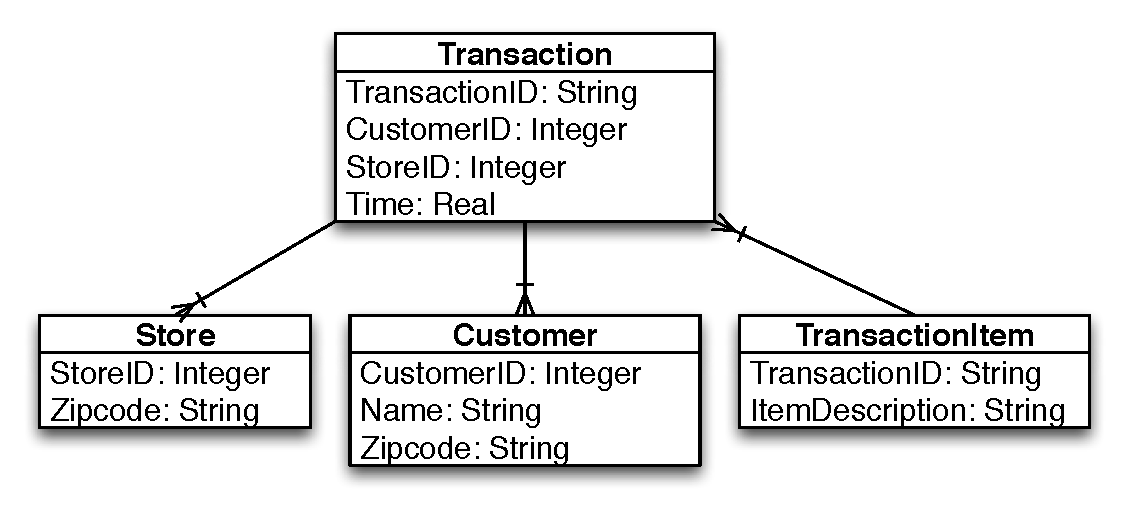
\includegraphics[width=3.5in]{figures/transactions_data_model.eps}
  \caption{Relational Data Model for Generated Data}
  \label{fig:relational-data-model}
\end{figure}

\subsection{Generation of Stores}
The locations of the stores are modeled by a probability density function (PDF) that gives the probability that a store's location is the given zip code. We designed the PDF to give to zip codes in high-population, high-income areas the highest probabilities. The PDF is composed of two individual PDFs. One PDF determines the probability of each zip code as the population of that zip code over the total population:

\begin{equation*}
p(\text{location}=z | \text{population}(z)) = \frac{\text{population}(z)}{\sum_{i} \text{population}(i)}
\end{equation*}

The second PDF scales the probabilities of the zip codes by their incomes.  The zip code with the highest-income has a probability $s$-times larger than that of the lowest-income zip code. The values in-between are interpolated using an exponential function:

\begin{equation*}
p(\text{location}=z | \text{income}(z)) = s ^ {\big( \frac{\text{income} - \min_i{\textrm{income}(i)}} {\max_i{\textrm{income}(i)} - \min_i{\textrm{income}(i)}} - 1 \big)}
\end{equation*}

The combined PDF is given as: 

\begin{align*}
p(\text{location}=z) = &Z p(\text{location}=z | \text{population}(z)) \\
&p(\text{location}=z | \text{income}(z))
\end{align*}

where $Z$ is the normalization factor.  Given the small size ($\approx$30,000 zip codes) of the data set, $Z$ can be found directly by iterating over all of the zip codes and summing the scores. The population and household income data for the zip codes were taken from from the U.S. Census American Community Survey \cite{ACS}.  The stores' locations are generated by sampling zip codes from the PDF.

\subsection{Generation of Customers}
For each proposed customer location zip code $z$, we compute the distance $d_m(z)$ between $z$ and each store's zip code $s_z$ to find the closest store.  The zip codes' latitudes and longitudes (taken from the Zip Code Database Project \cite{Zips}) are used to compute the distances. Each zip code $z$ is assigned a weight $w_z$ according to its distance $d_m(z)$ to the nearest store using an exponential distribution with the average distance $\beta$:

\begin{align*}
&w_z = \beta^{-1} \exp(-\beta^{-1} \, d_m(z)) \\
&d_m(z) = \min_{s_z} \, d(z, s_z)
\end{align*}

The customer's zip code is chosen by sampling from the zip codes with the probabiltiy of choosing each zip code $z$ proportional to its weight $w_z$.

Names are generated using data from the Name Database\cite{NameDB}. Each record in the database gives a name, a weight, and flag indicatings if the name can be used as a first name, a last name, or both.  PDFs generated for the first and last names using the weights.  The customer's name is generated by sampling a first name and a last name from each PDF respectively.

We determine the number of pets $N_p$ each customer has by sampling from a discrete uniform distribution of integers. We then sample the number of dogs $N_d$ as a discrete uniform distribution of integers between 0 and $N_p$.  The remaining number of pets are assigned to be cats.

\begin{align*}
N_c = N_p - N_d \\
N_d \sim U(0, N_p) \\
N_p \sim U(1, b)
\end{align*}

\subsection{Simulation of Transactions}
A transaction simulation is run for each customer. The transaction's store is set to the store located closest to the customer.  Transaction times are generated from a Monte Carlo process that proposes transaction times based on the usage of the customer's items and Poisson processes modeling the amount of time between the customer visiting the store and running out of the items (Section~\ref{sec:transaction-times}).  The purchased items are generated by a Hidden Markov Model (HMM) parameterized by the transaction time and amount of time remaining for the items in the customer's inventory (Section~\ref{sec:transaction-purchases}).

\begin{figure}[!t]
  \centering
  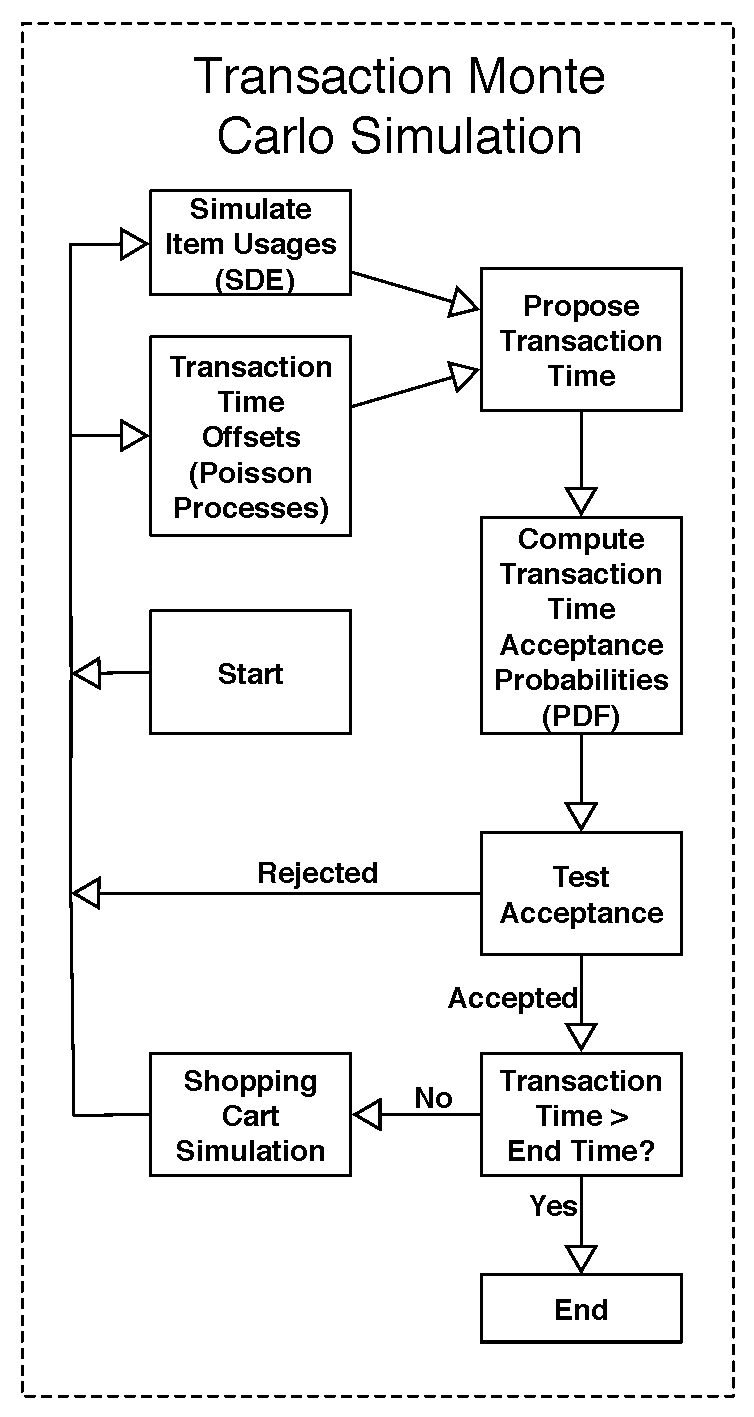
\includegraphics[width=3.5in]{figures/transaction_simulation.eps}
  \caption{Flowchart of Transaction Monte Carlo Simulation}
  \label{fig:trans_sim}
\end{figure}

\subsubsection{Simulation of Transaction Times} \label{sec:transaction-times}
Transaction times are simulated using a Monte Carlo method (Figure~\ref{fig:trans_sim}).  The usage over time of each item category is simulated. Items categories are groups of items which are interchangeable such as ``dry dog food,'' ``dry cat food,'' and ``kitty litter.'' The time between the customer's visit to the store to buy more items in each category and the exhaustion time of that item category is modeled using a Poisson process. Proposed transaction times for each item category are computed based on the exhaustion time and time sampled from the Poisson process. The earliest transaction time is taken as the overall proposed transaction time.  The probability of the transaction time is calculated using a PDF.  If rejected, new transaction times are proposed.  Otherwise, the purchased items are modeled using a separate process (discussed below). After the items are chosen, the process begins again with the simulation of the item category usages.

In the first stage of the process, the usage of items over time is modeled using a stochastic differential equation (SDE):

\begin{equation*}
\frac{da_i}{dt} = \min \{-\mu_i + \sigma_i\, dW_i(t), 0\}
\end{equation*}

where $a_i$ is the amount of item category $i$ ``stuff'' remaining at time $t$. The variable $\mu_i$ gives the average usage rate and $\sigma^2_i$ gives the variance of the usage rate for item category $i$. The SDE is numerically integrated using the Euler-Maruyama method\cite{Klouden13} with time step $\Delta t_n$ sampled from an exponential distribution:

\begin{align*}
&a_{n+1, i} = a_{n,i} - \min \{\mu_{i, c} \, \Delta t_n + \sigma_{i, c} \, \sqrt{\Delta t_n} R_n, 0.0\} \\
&t_{n+1} = t_n + \Delta t_n \\
&\Delta t_n \sim \text{Exp}(\beta^{-1}_{i,c}) \\
&R_n \sim \text{N}(0, 1)
\end{align*}

where $a_{n, i}$ is the amount remaining of item category $i$ at time step $t_n$, $\mu_{i,c}$ is the average amount used per time used, $\sigma^2_{i,c}$ is the variance of the amount used per time used, and $\beta_{i,c}$ is the item category's average amount of time between uses for customer $c$.  The parameters $\mu_{i, c}$, and $\sigma^2_{i,c}$ are computed from a base rate for each item category multiplied by the number of pets of the appropriate species the customer $c$ has.  The exhaustion time $T_{E,i}$ for each item category is found by simulating the usage until $a_{n,i} \leq 0$.

The proposed transaction time is found from the exhaustion times (Eq.~\ref{eq:transaction-times}).  For each item category, the offset time $T_{O, i}$ between when a customer would visit the store and the exhaustion time is sampled from an exponential distribution. The distribution is parameterized by $\beta_c$, the average number of days before triggering a transaction. The parameter $\beta_c$ is set separately for each customer $c$ by sampling from a uniform distribution. A proposed transaction time $T_{P, i}$ for each item category is found by subtracting the offset time $T_{O, i}$ from the exhaustion time $T_{E, i}$.  The earliest proposed transaction time is taken as the overall proposed transaction time $T_T$.

\begin{align} \label{eq:transaction-times}
&T_T = \min_i \, \{  T_{P, i}\} \\
&T_{P, i} = T_{E,i} - T_{O, i} \nonumber\\
&T_{O, i} \sim \text{Exp}(\beta^{-1}_c) \nonumber \\
&\beta_c \sim \text{U}(a, b) \nonumber
\end{align}

The acceptance probability $p(t_{n+1}=T_T|t_n)$ of the proposed transaction time $T_T$ is modeled using a PDF (Eq.~\ref{eq:transaction_time_pdf}). For now, the PDF only ensures that the proposed transaction time is more recent than the last transaction time.

%The PDF could be extended to incorporate additional factors including time-dependent events such as sales, weather, and the amount of money the customer has available at the time.

\begin{equation} \label{eq:transaction_time_pdf}
p(t_{n+1}=T_T|t_n) = \left\{ 
  \begin{array}{l l}
   1 & \quad t_{n+1} \geq t_n\\
   0 & \quad t_{n+1} < t_n
  \end{array} \right.
\end{equation}

The proposed transaction time is accepted if $p(t_{n+1}=T_T) < r$, where $r \sim \text{U}(0, 1)$. Until the proposed transaction time is accepted, a new proposed transaction time is generated by sampling new offset times. If the proposed transaction time is accepted, the purchased items are chosen through a separate simulation discussed in Section~\ref{sec:transaction-purchases} below. Transactions are generated until the accepted transaction time is later than the end time given as a simulation parameter.

\begin{figure*}[!t]
  \centering
  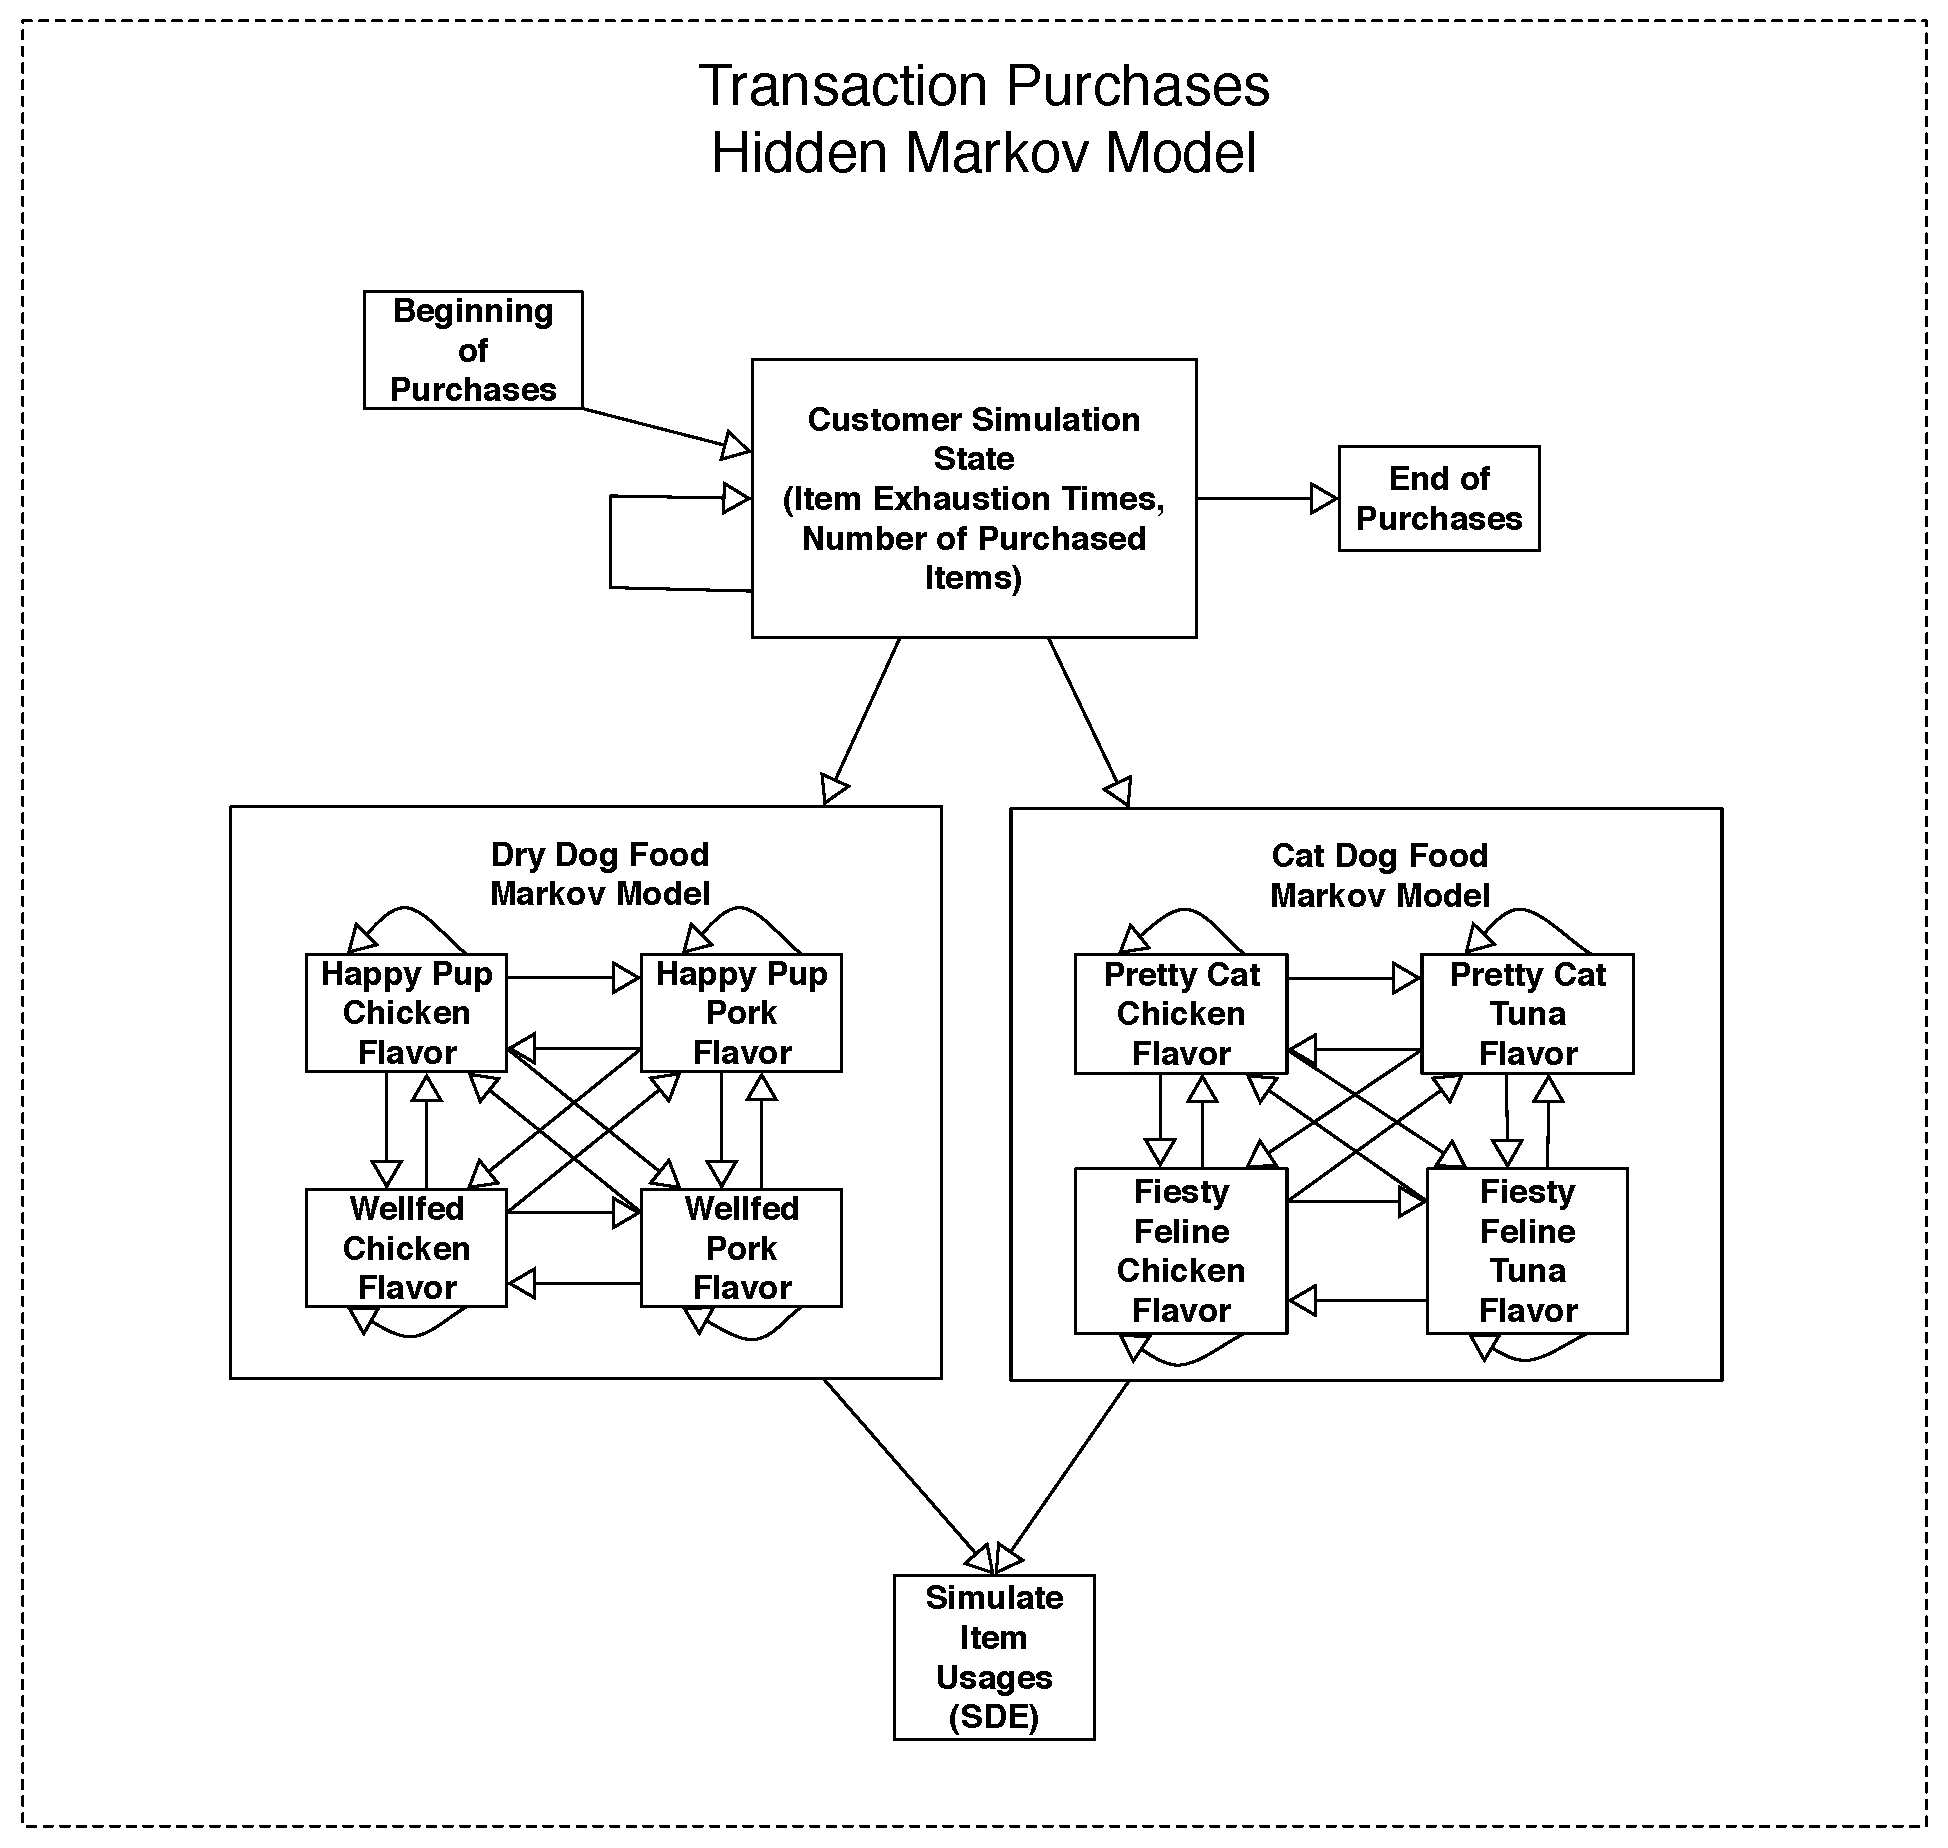
\includegraphics[width=6in]{figures/shopping_cart_simulation.eps}
  \caption{Example Shopping Cart Hidden Markov Model}
  \label{fig:shopping_cart_sim}
\end{figure*}

\subsubsection{Simulation of Transaction Items} \label{sec:transaction-purchases}

A customer's purchases in each transaction are modeled using a layered Hidden Markov Model (HMM) (Figure~\ref{fig:shopping_cart_sim}).  The HMM has three types of states: the start state, the purchase states, and the stop state. There are an infinite number of purchase states, parameterized by the exhaustion times of the customer's item categories and the transaction time.

The observables of the states correspond to the item categories.  Each item category $i$ is assigned a weight $w_i$ according to the amount of time between the transaction time $T_t$ and $T_{E,i}$ when each item category will be exhausted (based on the usage simulations):

\begin{align} \label{eq:category-weights}
&w_i = - \beta^{-1}_c \exp(-\beta^{-1}_c (T_{E, i}- T_T)) \\
&\beta^{-1}_c \sim U(a,b) \nonumber
\end{align}

where $\beta_c$ the average number of days between when a customer purchases an item and the exhaustion time. The value $\beta_c$ is set separately for each customer by sampling from a uniform distribution. The value $w_i$ is used to model the propensity for a customer to purchase an item they will run out at time $T_{E, i}$ in the future when at the store at time $T_T$.

The item category is chosen by sampling from the item categories with the probability of choosing each item category $i$ proportional to its weight $w_i$.

Markov Models are used to model the customer's purchasing behavior for each item category.  Each state $X_n$ corresponds to an item in that category. The customer's buying habits are determined by the transition probabilities:  

\begin{align}
Pr(X_{n+1}&=x|X_n=y) = \nonumber \\
& \left\{ 
  \begin{array}{l l}
   (1.0 - p_l) \, Pr(x,y)  & \quad \text{if $x \neq y$}\\
   p_l & \quad \text{if $x = y$}
  \end{array} \right.
\end{align}

where $w_l$ is the loopback probability, giving the probability of choosing the same item $y$ again. The function $Pr(x,y)$ gives the probability of choosing the item $x$ given that the previous item was $y$:

\begin{equation*}
Pr(x,y) = \frac{\sum_f w_f w_{f,s}(x, y)}{\sum_{j \neq x} \sum_f w_f w_{f,s}(x, j)}
\end{equation*}

where $w_f$ is the weight of a particular field $f$.   The pair of items $x$ and $y$ are weighted  according to the equality of the values for each field:

\begin{equation*}
w_{f,s}(x,y) = \left\{ 
  \begin{array}{l l}
   w_{f,s}  & \quad \text{if $x$.$f$ = $y$.$f$}\\
   1 - w_{f, s} & \quad \text{if $x$.$f$ $\neq$ $y$.$f$}
  \end{array} \right.
\end{equation*} 

The weights $w_l$, $w_f$, and $w_{f, s}$ are chosen randomly for each customer:

\begin{align*}
&w_l \sim N(\mu, \sigma^2) \\
&w_f \sim N(\mu, \sigma^2) \\
&w_{f, s} \sim N(\mu, \sigma^2)
\end{align*}

If the weights are greater than 1, they are rounded down to 1.  Likewise, if the weights are less than 0, they are rounded up to 0.

%\textcolor{red}{reorder so that probilities describe habits}

%For example, if a customer tends to buy the same brand of dog food repeatedly, the outgoing edges to all products of the same brand as the product in the current state will be higher than those for other brands' products. If the customer does not care about flavor, the outgoing edges to all products from the current brand will be equal, otherwise the edge weights can be adjusted to prefer a specific combination of brand and flavor.  Likewise, if a customer cares more about flavor or cost, the edge weights will be assigned appropriately.

To simulate an item purchase, the chosen Markov model is transitioned forward by one state. The current states of the Markov models are kept between purchases.  After an item is chosen, the item category's exhaustion time is updated by propagating the item category usage SDE described in Section~\ref{sec:transaction-times}, resulting in an implicit creation of the next possible purchase state in the HMM.

After each purchase, the HMM's current state is transitioned to either the new purchase state or the stop state.  The probability of choosing the next state is 

\begin{align*}
&Pr(X_{n+1}=\text{stop}|X_n) = p(\text{stop})\\
&Pr(X_{n+1}=\text{purchase}|X_n) = 1 - p(\text{stop})
\end{align*}

where $p(\text{stop})$ is the probability of choosing the stop state and is given by

\begin{equation*}
 p(\text{stop}) = \frac{w_{\text{stop}}}{w_{\text{stop}} + \sum_i w_i}
\end{equation*}

where $w_{\text{stop}}$ is the weight of the stop state and is a simulation parameter and the weight $w_i$ of each item category $i$ was given earlier in Eq.~\ref{eq:category-weights}.

If the stop state is chosen, the transaction is finished and the next transaction is started according to the procedure presented in Section~\ref{sec:transaction-times}.

%The HMM can be extended to consider additional factors such as the amount of money spent so far in the transaction and the customer's spending habits.

\section{Implementation}
The models and simulations were implemented using Python. The source code is available at \url{https://github.com/rnowling/bigpetstore-data-generator} under the Apache Public License v2.

\section{Evaluation of the Model}
In accordance with our original design goals, we evaluated the model and implementation in terms of their abilities to generate semantically-interesting data and scale from a single local machine to a cluster.

\subsection{Example Analysis of Generated Data}
To evaluate the semantic content of the generated data, we performed two example analyses in support of a fictional advertising campaign using data for 10 stores, 10,000 customers, and five years of transactions generated from the model. The analyses were designed to be realistic and driven by real-world business concerns.  Due to limited advertising budgets, businesses need to decide who to target and what sort of advertisements are likely to be effective for each type of customer.  We analyzed data generated from the model to determine where the advertising campaigns should be targeted geographically and identify customer purchasing profiles.

First, we wanted to identify how close most customers live to a store since advertising to people who live or work too far away from a store is unlikely to be effective and will increase our costs. We analyzed the distribution of distances between customers' homes and their nearest stores.  We found that most customers tend to live within 15 miles of their closest store, suggesting that we should limit our advertising to a 15-mile radius around each our store.

\begin{figure}[!t]
  \centering
  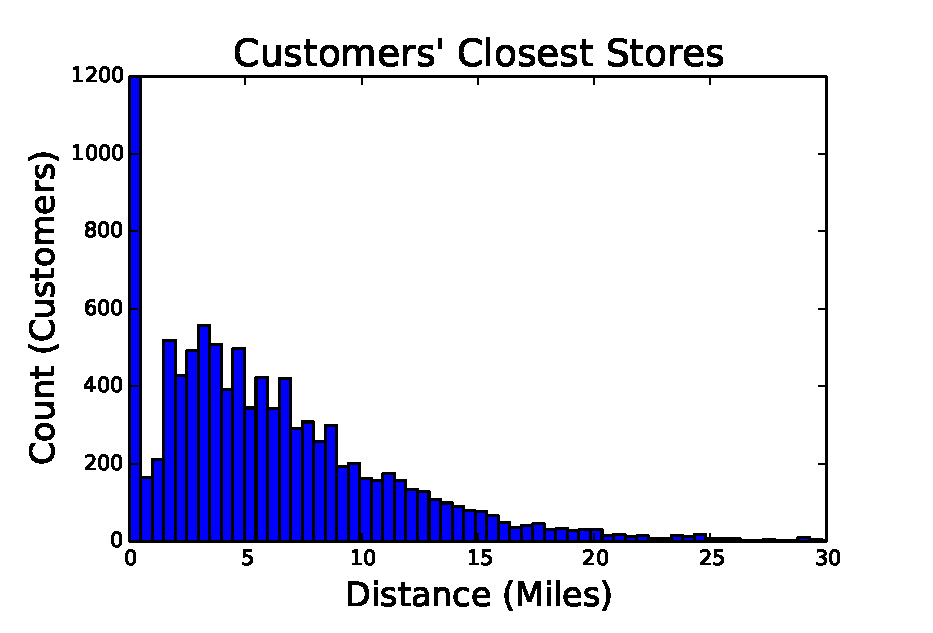
\includegraphics[width=3.5in]{figures/customer_store_distances.eps}
  \caption{Distributions of Distances of Customers to Closest Stores}
  \label{fig:cluster_analysis}
\end{figure}

Secondly, we profiled our customers' purchasing habits to optimize the advertising campaign's effectiveness by customizing the advertised products for each customer.  For each customer, we generated a feature vector by computing the frequency with which they would purchase the same brand or flavor from one transaction to the next.  We clustered the customers' feature vectors using the KMeans algorithm with a range of cluster counts. Twenty clusters converged the error.

\begin{figure}[!t]
  \centering
  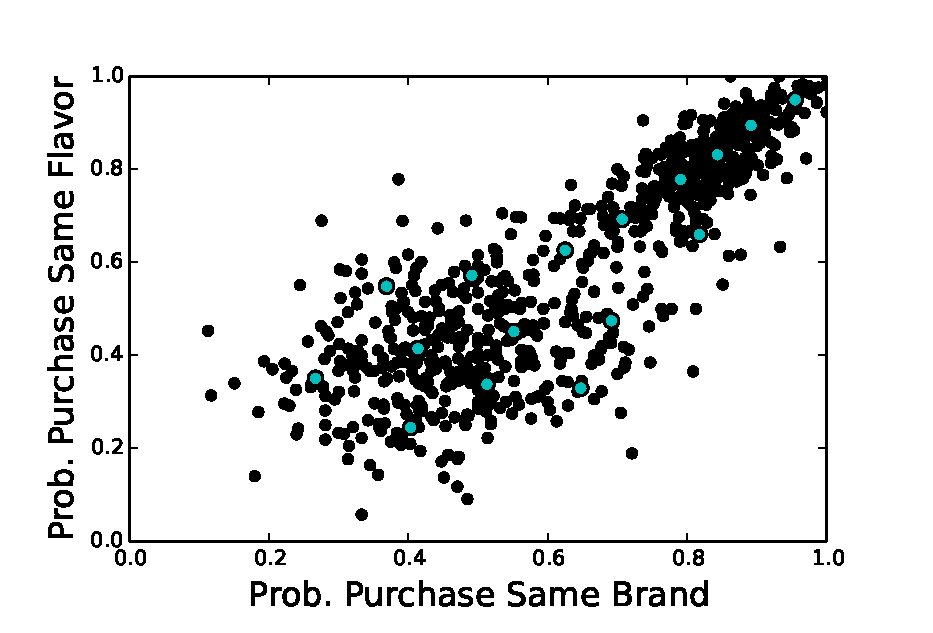
\includegraphics[width=3.5in]{figures/cluster_analysis.eps}
  \caption{Clustering of Brand and Flavor Purchasing Preferences. Grey plus signs (+) represent customer data points, and cyan circles represent cluster centers.}
  \label{fig:cluster_analysis}
\end{figure}

Analysis of the feature vectors and clusters revealed four predominant purchasing profiles (Figure~\ref{fig:cluster_analysis}).  High frequencies of purchasing the same flavors repeatedly were tightly-correlated with high frequencies of purchasing the same brands -- these customers were likely to be happy with a particular item and kept purchasing the same item repeatedly.  For our advertising campaign, it would be unlikely to get these customers to purchase different items, so we should create incentives to purchase larger quantities, especially when inventory levels are high and needed to be depleted.  Other customers had a tendency to purchase either the same flavor or brand repeatedly, but varied in their choice of the other.  For customers who prefer a particular brand, we should target our advertising campaign to suggest other flavors sold by that brand.  Likewise, for customers who prefer a particular flavor, we should target our advertising campaign to suggest other brands with that flavor.  Lastly, some customers had very low frequencies of purchasing neither the same brand nor flavor.  Other factors, such as cost, not represented in this analysis may be driving these customers' purchasing habits and will need further study.


\subsection{Scaling of Data Size and Run Time}
BigPetStore aims to scale from a local desktop to a large cluster. To evaluate the scaling of the model and implementation, we benchmarked the data generator on a laptop with a 2 GHz Intel Core i7 CPU, 8 GB of RAM, and a 256 GB SSD using the Python implementation with a single thread. Using the test setup, between 1,500 and 2,000 transactions can be generated per second (Table~\ref{tab:benchmarks}). As the customers' transaction simulations are independent of one another, the transaction generation can easily be parallelized so that 1,500-2,000 transactions can be generated per thread per second.

\begin{table}[!t]
%% increase table row spacing, adjust to taste
\renewcommand{\arraystretch}{1.3}
% if using array.sty, it might be a good idea to tweak the value of
% \extrarowheight as needed to properly center the text within the cells
\caption{Benchmarks of Data Generator}
\label{tab:benchmarks}
\centering
%% Some packages, such as MDW tools, offer better commands for making tables
%% than the plain LaTeX2e tabular which is used here.
\begin{tabular}{|p{0.75cm}||p{1.2cm}||p{1cm}||p{1.25cm}||p{1cm}||p{1cm}|}
\hline
Stores & Customers & Simulated Time (years) & Transactions & Data Size (MB) & Run Time (min)\\ \hline
10 & 10,000 & 1 & 279,870 & 18 & 3.5 \\ \hline
%10 & 100,000 & 1 & 
100 & 10,000 & 1 & 279,586 & 18 & 3.5 \\ \hline
% 100 & 100,000 & 1 & 
10 & 1,000 & 5 & 123,309 & 8 & 1.1 \\ \hline
100 & 1,000 & 5 & 127,064 & 8 & 1.2 \\ \hline
10 & 10,000 & 5 & 1,275,542 & 84 & 11.0 \\ \hline
%10 & 100,000 & 5 & 
100 & 10,000 & 5 & 1,268,403 & 84 & 10.5 \\ \hline
\end{tabular}
\end{table}

The number of transactions (and hence, data size) grows as $O(N_c T)$ where $N_c$ is the number of customers and $T$ is the amount of time to be simulated. The amount of data generated can be scaled as large as necessary simply by increasing $N_c$ and $T$. Five years of transactions for 100,000 customers will generate approximately 1 GB of data. A terabyte of data can be generated by simulating 100 million customers over five years. 

\section{Discussion and Conclusion}
We have described a domain-driven mathematical model and accompanying simulation for generating semantically-rich data.  We validated the method by analyzing generated data to inform decisions in a fictional advertising campaign. Scalability testing combined with analysis of the implementation suggests that the data generation method can scale from small data sets appropriate for desktop development to large data sets for testing and benchmarking of clusters. We have released the implementation source code under the open-source Apache Public License v2.

We see many opportunities for building on the work presented.  We intend to expand the model to incorporate additional factors.  Deeper integration of existing fields such as location and purchasing profiles (e.g., to model regional purchasing preferences) will increase the variety of the semantic information encoded in the generated data. The incorporation of weather and climate data can be used to influence when customers shop, the types of products they buy, and the amount of products purchased. For example, customers would be less likely to shop during snow storms, more likely to buy items such as winter apparel for their pets, and more likely to purchase bulk quantities to reduce the number of transactions. Modeling of time-dependent events such as sales, evolution of customer purchasing profiles over time, and ``life events,'' such as the birth or passing of pets, will enable more interesting time-series analysis of the data.  We would also like to expand the scope of the model to incorporate business processes (such as inventory management, customer complaints, employees, etc.), thus enabling queries about the relationship between internal business process and customer behavior.

The current implementation was prototyped in Python.  We are working to implement the model using Hadoop and Spark.  We will commit the resulting implementations to BigPetStore hosted in the Apache BigTop distribution to enable ease of access and immediate benefit to current users. 


% no \IEEEPARstart
%This demo file is intended to serve as a ``starter file''
%for IEEE conference papers produced under \LaTeX\ using
%IEEEtran.cls version 1.7 and later.
% You must have at least 2 lines in the paragraph with the drop letter
% (should never be an issue)
%I wish you the best of success.

%\hfill mds
 
%\hfill January 11, 2007


% An example of a floating figure using the graphicx package.
% Note that \label must occur AFTER (or within) \caption.
% For figures, \caption should occur after the \includegraphics.
% Note that IEEEtran v1.7 and later has special internal code that
% is designed to preserve the operation of \label within \caption
% even when the captionsoff option is in effect. However, because
% of issues like this, it may be the safest practice to put all your
% \label just after \caption rather than within \caption{}.
%
% Reminder: the "draftcls" or "draftclsnofoot", not "draft", class
% option should be used if it is desired that the figures are to be
% displayed while in draft mode.
%
%\begin{figure}[!t]
%\centering
%\includegraphics[width=2.5in]{myfigure}
% where an .eps filename suffix will be assumed under latex, 
% and a .pdf suffix will be assumed for pdflatex; or what has been declared
% via \DeclareGraphicsExtensions.
%\caption{Simulation Results}
%\label{fig_sim}
%\end{figure}

% Note that IEEE typically puts floats only at the top, even when this
% results in a large percentage of a column being occupied by floats.


% An example of a double column floating figure using two subfigures.
% (The subfig.sty package must be loaded for this to work.)
% The subfigure \label commands are set within each subfloat command, the
% \label for the overall figure must come after \caption.
% \hfil must be used as a separator to get equal spacing.
% The subfigure.sty package works much the same way, except \subfigure is
% used instead of \subfloat.
%
%\begin{figure*}[!t]
%\centerline{\subfloat[Case I]\includegraphics[width=2.5in]{subfigcase1}%
%\label{fig_first_case}}
%\hfil
%\subfloat[Case II]{\includegraphics[width=2.5in]{subfigcase2}%
%\label{fig_second_case}}}
%\caption{Simulation results}
%\label{fig_sim}
%\end{figure*}
%
% Note that often IEEE papers with subfigures do not employ subfigure
% captions (using the optional argument to \subfloat), but instead will
% reference/describe all of them (a), (b), etc., within the main caption.


% An example of a floating table. Note that, for IEEE style tables, the 
% \caption command should come BEFORE the table. Table text will default to
% \footnotesize as IEEE normally uses this smaller font for tables.
% The \label must come after \caption as always.
%
%\begin{table}[!t]
%% increase table row spacing, adjust to taste
%\renewcommand{\arraystretch}{1.3}
% if using array.sty, it might be a good idea to tweak the value of
% \extrarowheight as needed to properly center the text within the cells
%\caption{An Example of a Table}
%\label{table_example}
%\centering
%% Some packages, such as MDW tools, offer better commands for making tables
%% than the plain LaTeX2e tabular which is used here.
%\begin{tabular}{|c||c|}
%\hline
%One & Two\\
%\hline
%Three & Four\\
%\hline
%\end{tabular}
%\end{table}


% Note that IEEE does not put floats in the very first column - or typically
% anywhere on the first page for that matter. Also, in-text middle ("here")
% positioning is not used. Most IEEE journals/conferences use top floats
% exclusively. Note that, LaTeX2e, unlike IEEE journals/conferences, places
% footnotes above bottom floats. This can be corrected via the \fnbelowfloat
% command of the stfloats package.



% \section{Conclusion}
%The conclusion goes here.




% conference papers do not normally have an appendix


% use section* for acknowledgement
\section*{Acknowledgment}
The authors would like to thank Brian P. Clare and Casey Robinson for useful and interesting discussion.  JV would like to thank the Apache BigTop community for their interest in and support of BigPetStore.  We would also like to thank Matt Fenwick, Nigel Savage, and Bhashit Parikh for their contributions to BigPetStore. The authors would like to thank Red Hat, Inc. and the University of Notre Dame for their support of this work.





% trigger a \newpage just before the given reference
% number - used to balance the columns on the last page
% adjust value as needed - may need to be readjusted if
% the document is modified later
%\IEEEtriggeratref{8}
% The "triggered" command can be changed if desired:
%\IEEEtriggercmd{\enlargethispage{-5in}}

% references section

% can use a bibliography generated by BibTeX as a .bbl file
% BibTeX documentation can be easily obtained at:
% http://www.ctan.org/tex-archive/biblio/bibtex/contrib/doc/
% The IEEEtran BibTeX style support page is at:
% http://www.michaelshell.org/tex/ieeetran/bibtex/
\bibliographystyle{IEEEtran}
% argument is your BibTeX string definitions and bibliography database(s)
\bibliography{IEEEabrv,paper}
%\bibliography{paper}
%
% <OR> manually copy in the resultant .bbl file
% set second argument of \begin to the number of references
% (used to reserve space for the reference number labels box)
%\begin{thebibliography}{1}

%\bibitem{IEEEhowto:kopka}
%\subsection{Subsection Heading Here}
%Subsection text here.


%\subsubsection{Subsubsection Heading Here}
%Subsubsection text here.
%H.~Kopka and P.~W. Daly, \emph{A Guide to \LaTeX}, 3rd~ed.\hskip 1em plus
%  0.5em minus 0.4em\relax Harlow, England: Addison-Wesley, 1999.

%\end{thebibliography}




% that's all folks
\end{document}


